\titlepageframe % Specific command

% OBJETIVOS %

\begin{tframe}{Objetivos}
	\begin{itemize}
			\item Crear las bases, extendibles y genéricas, de un videojuego \textit{roguelike}
			\item Añadir elementos de accesibilidad, en especial para invidentes
	\end{itemize}
\end{tframe}

% QUÉ ES UN ROGUELIKE %

\begin{tframe}{Objetivos}
	\begin{itemize}
			\item<+-| alert@+> Crear las bases, extendibles y genéricas, de un videojuego \textit{roguelike}
			\item Añadir elementos de accesibilidad, en especial para invidentes
	\end{itemize}
\end{tframe}

\begin{tframe}{¿Qué es un \textit{roguelike}?}
	Género de videojuegos que suele contener los siguientes elementos:
	\begin{itemize}
		\item<+-| alert@+> Gran dificultad
			\begin{itemize}
				\item Muerte permanente o \textit{permadeath}
				\item Escalable en base al jugador
			\end{itemize}
	\end{itemize}
\end{tframe}

\begin{tframe}{¿Qué es un \textit{roguelike}?}
	Género de videojuegos que suele contener los siguientes elementos:
	\begin{itemize}
		\item Gran dificultad
			\begin{itemize}
				\item Muerte permanente o \textit{permadeath}
				\item Escalable en base al jugador
			\end{itemize}
		\item<+-| alert@+> Aleatoriedad
		\begin{itemize}
			\item Mapas
			\item Enemigos
			\item Objetos
		\end{itemize}
	\end{itemize}
\end{tframe}

\begin{tframe}{¿Qué es un \textit{roguelike}?}
	Género de videojuegos que suele contener los siguientes elementos:
	\begin{itemize}
		\item Gran dificultad
			\begin{itemize}
				\item Muerte permanente o \textit{permadeath}
				\item Escalable en base al jugador
			\end{itemize}
		\item Aleatoriedad
		\begin{itemize}
			\item Mapas
			\item Enemigos
			\item Objetos
		\end{itemize}
			\item<+-| alert@+> Exploración
	\end{itemize}
\end{tframe}

% Roguelike en nuestro proyecto %

\begin{tframe}{Elementos \textit{roguelike} en nuestro proyecto}
	En nuestro proyecto tenemos las siguientes características:
	\begin{itemize}
		\item<+-| alert@+> Gran dificultad
			\begin{itemize}
				\item Diferentes clases de enemigos que se adaptan al nivel del usuario
				\item Enemigos con distintas IAs
			\end{itemize}
	\end{itemize}
\end{tframe}

\begin{tframe}{Elementos \textit{roguelike} en nuestro proyecto}
	En nuestro proyecto tenemos las siguientes características:
	\begin{itemize}
		\item Gran dificultad
			\begin{itemize}
				\item Diferentes clases de enemigos que se adaptan al nivel del usuario
				\item Enemigos con distintas IAs
			\end{itemize}
		\item<+-| alert@+> Aleatoriedad
		\begin{itemize}
			\item Aleatoriedad en mapa y habitaciones
			\item Generador de encuentros: enemigos y objetos
		\end{itemize}
	\end{itemize}
\end{tframe}

\begin{tframe}{Elementos \textit{roguelike} en nuestro proyecto}
	En nuestro proyecto tenemos las siguientes características:
	\begin{itemize}
		\item Gran dificultad
			\begin{itemize}
				\item Diferentes clases de enemigos que se adaptan al nivel del usuario
				\item Enemigos con distintas IAs
			\end{itemize}
		\item Aleatoriedad
		\begin{itemize}
			\item Aleatoriedad en mapa y habitaciones
			\item Generador de encuentros: enemigos y objetos
		\end{itemize}
		\item<+-| alert@+> Exploración
		\begin{itemize}
			\item Nuevos objetos
			\item Encontrar la salida
		\end{itemize}
	\end{itemize}
\end{tframe}

% NO ES NADA DIFERENTE %

\begin{tframe}{Otros \textit{roguelikes} con las mismas ideas}
	FTL (Faster Than Light). 2012.
	\begin{figure}[h]
		
\includegraphics[width=8cm]{../img/ftl}
	\end{figure}
\end{tframe}

\begin{tframe}{Otros \textit{roguelikes} con las mismas ideas}
	Enter the gungeon. 2016.
	\begin{figure}[h]
		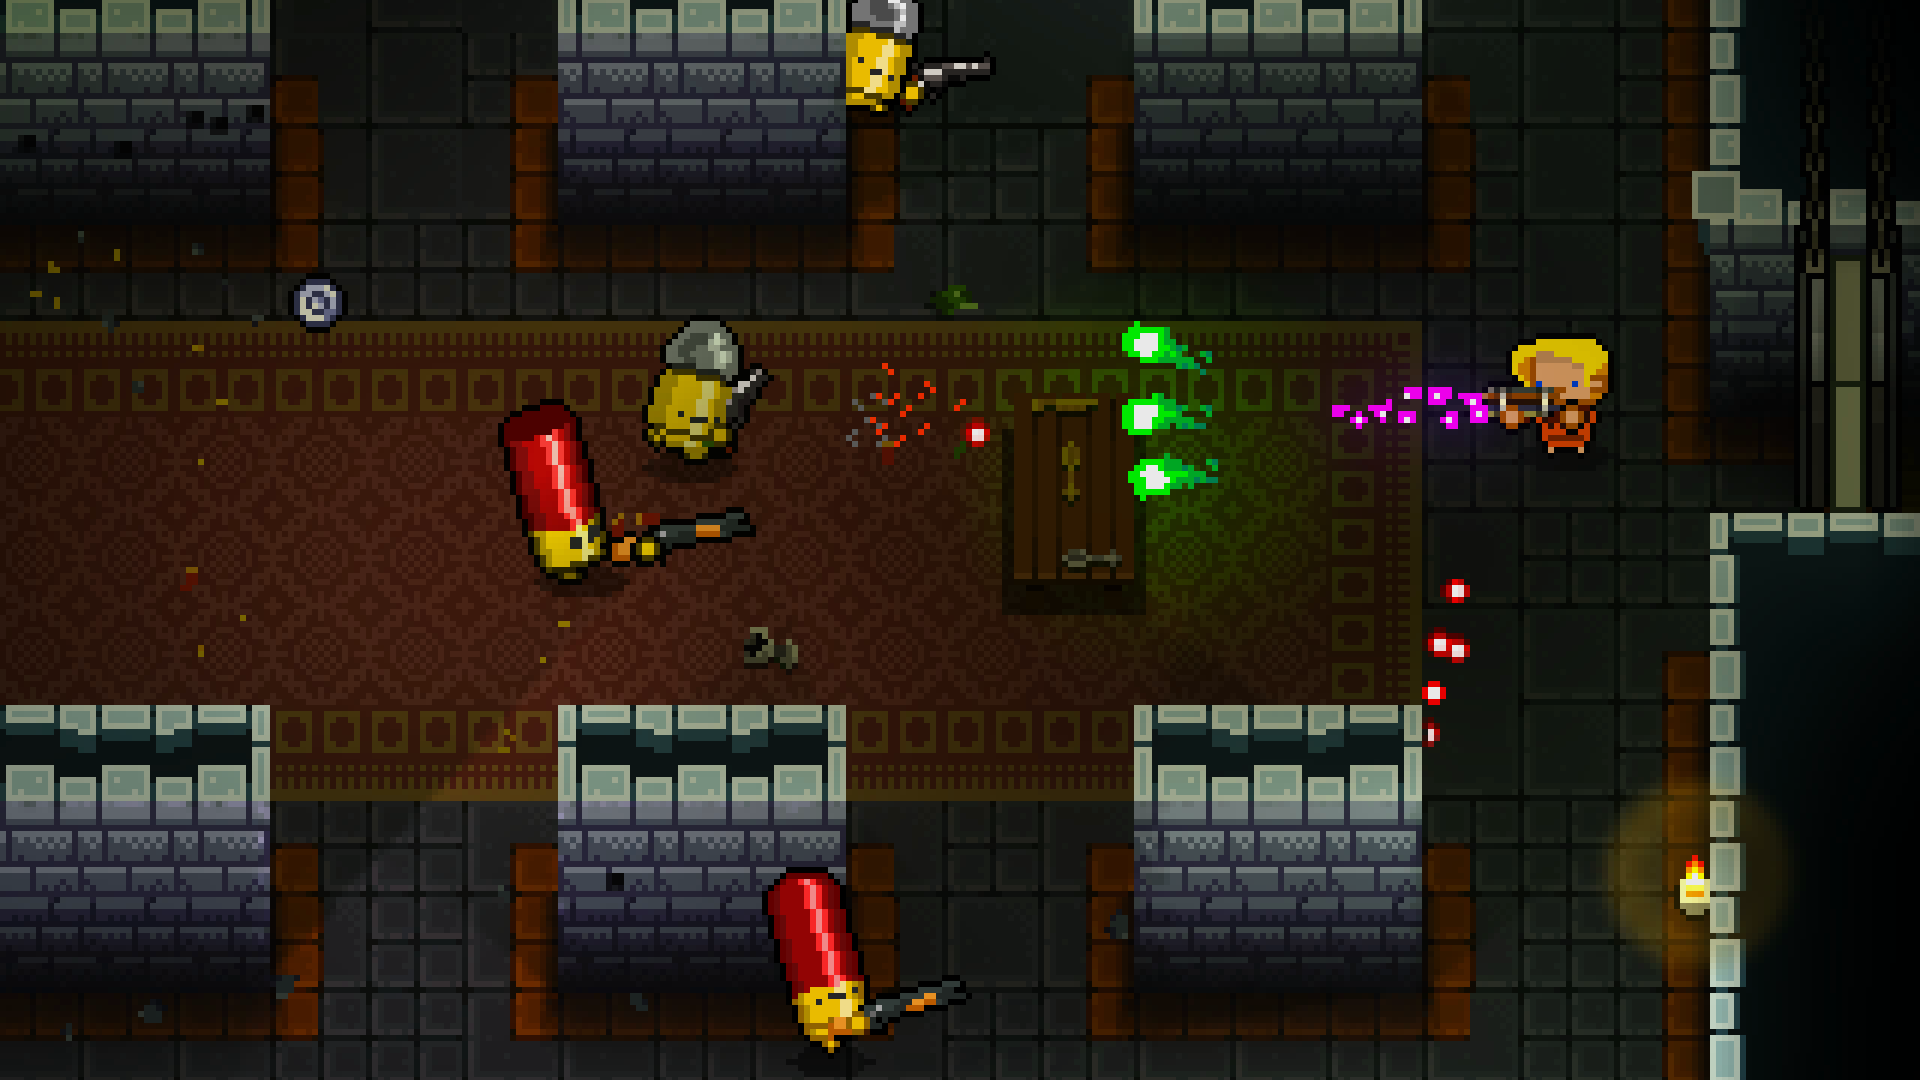
\includegraphics[width=8cm]{../img/enterthegungeon}
	\end{figure}
\end{tframe}

% POR QUÉ DISCRIMINAR? %

\begin{tframe}{Objetivos}
	\begin{itemize}
		\item Crear las bases, extendibles y genéricas, de un videojuego \textit{roguelike}
		\item<+-| alert@+> Añadir elementos de accesibilidad, en especial para invidentes
	\end{itemize}
\end{tframe}

\begin{tframe}{¿Por qué discriminar?}
	\begin{itemize}
			\item<+-| alert@+> Limitar el campo de visión (FOV)	
	\end{itemize}
\end{tframe}

\begin{tframe}{¿Por qué discriminar?}
	\begin{itemize}
		\item Limitar el campo de visión (FOV)
		\item<+-| alert@+> No poder cambiar las teclas a usar
	\end{itemize}
\end{tframe}

\begin{tframe}{¿Por qué discriminar?}
	\begin{itemize}
		\item Limitar el campo de visión (FOV)
		\item No poder cambiar las teclas a usar
		\item<+-| alert@+> Obligar al jugador a distinguir colores para progresar
	\end{itemize}
\end{tframe}

% ELEMENTOS DE ACCESIBILIDAD EN NUESTRO PROYECTO %

\begin{tframe}{Elementos de accesbilidad en nuestro proyecto}
	\begin{itemize}
		\item<+-| alert@+> Posibilidad de cambiar las teclas (\textit{rebindable keys})
	\end{itemize}
\end{tframe}

\begin{tframe}{Elementos de accesbilidad en nuestro proyecto}
	\begin{itemize}
		\item Posibilidad de cambiar las teclas (\textit{rebindable keys})
		\item<+-| alert@+> Tamaño de letra grande para facilitar la lectura
	\end{itemize}
\end{tframe}

\begin{tframe}{Elementos de accesbilidad en nuestro proyecto}
	\begin{itemize}
		\item Posibilidad de cambiar las teclas (\textit{rebindable keys})
		\item Tamaño de letra grande para facilitar la lectura
		\item<+-| alert@+> Elementos en la interfaz distinguibles, no solamente por color, pero también forma
	\end{itemize}
\end{tframe}

\begin{tframe}{Elementos de accesbilidad en nuestro proyecto}
	\begin{itemize}
		\item Posibilidad de cambiar las teclas (\textit{rebindable keys})
		\item Tamaño de letra grande para facilitar la lectura
		\item Elementos en la interfaz distinguibles, no solamente por color, pero también forma
		\item<+-| alert@+> Posibilidad de cambiar la paleta de colores
	\end{itemize}
\end{tframe}

\begin{tframe}{Elementos de accesbilidad en nuestro proyecto}
	\begin{itemize}
		\item Posibilidad de cambiar las teclas (\textit{rebindable keys})
		\item Tamaño de letra grande para facilitar la lectura
		\item Elementos en la interfaz distinguibles, no solamente por color, pero también forma
		\item Posibilidad de cambiar la paleta de colores
		\item<+-| alert@+> Soporte para invidentes
	\end{itemize}
\end{tframe}

% NUESTROS OBJETIVOS PARA DAR SOPORTE A INVIDENTES %

\begin{tframe}{Objetivos para dar soporte a invidentes}
	\begin{itemize}
		\item<+-| alert@+> Generar frases que describan todo lo que el jugador necesita		
	\end{itemize}
\end{tframe}

\begin{tframe}{Objetivos para dar soporte a invidentes}
	\begin{itemize}
		\item Generar frases que describan todo lo que el jugador necesita
		\item<+-| alert@+> Evitar que dichas frases sean muy repetitivas
	\end{itemize}
\end{tframe}

\begin{tframe}{Objetivos para dar soporte a invidentes}
	\begin{itemize}
		\item Generar frases que describan todo lo que el jugador necesita
		\item Evitar que dichas frases sean muy repetitivas
		\item<+-| alert@+> Tener en cuenta la temporalidad
	\end{itemize}
\end{tframe}

\begin{tframe}{Objetivos para dar soporte a invidentes}
	\begin{itemize}
		\item Generar frases que describan todo lo que el jugador necesita
		\item Evitar que dichas frases sean muy repetitivas
		\item Tener en cuenta la temporalidad
		\item<+-| alert@+> Crearlo lo más extensible/fácilmente posible
	\end{itemize}
\end{tframe}

\begin{tframe}{Objetivos para dar soporte a invidentes}
	\begin{itemize}
		\item Generar frases que describan todo lo que el jugador necesita
		\item Evitar que dichas frases sean muy repetitivas
		\item Tener en cuenta la temporalidad
		\item Crearlo lo más extensible/fácilmente posible
		\item<+-| alert@+> No dejar de lado al usuario vidente
	\end{itemize}
\end{tframe}

% ¿CÓMO GENERAR FRASES AUTOMÁTICAMENTE/ALEATORIAMENTE? %

\begin{tframe}{¿Cómo generamos las frases automáticamente?}
	\begin{itemize}
		\item Gramáticas
		\item Diccionarios
	\end{itemize}
\end{tframe}

\begin{tframe}{¿Cómo generamos las frases automáticamente?}
	\begin{itemize}
		\item<+-| alert@+> Gramáticas
		\item Diccionarios
	\end{itemize}
\end{tframe}

\begin{frame}[t, fragile]{Gramáticas}
	\vspace*{\fill}
	\begin{Verbatim}
El    héroe   coge   la   espada   metálica
	\end{Verbatim}
	\vspace*{\fill}
\end{frame}

\begin{frame}[t, fragile]{Gramáticas}
	\vspace*{\fill}
	\begin{Verbatim}
El    héroe   coge   la   espada   metálica
	\end{Verbatim}
	\begin{verbatim}
		DET     S       V     D     S        ADJ
	\end{verbatim}
	\vspace*{\fill}
\end{frame}

\begin{frame}[t, fragile]{Gramáticas}
En inglés:

	\begin{Verbatim}
The     hero   picks    the    metallic    sword
	\end{Verbatim}
	\begin{Verbatim}
DET       S      V        D        ADJ       S
	\end{Verbatim}
\vspace*{12px}
En español:
	\begin{Verbatim}
El    héroe   coge   la   espada   metálica
	\end{Verbatim}
	\begin{Verbatim}
DET     S       V     D     S        ADJ
	\end{Verbatim}
\end{frame}

\begin{frame}[t, fragile]{Gramáticas}
Estas gramáticas las especificamos en un archivo JSON, que dependerá del idioma:
	\begin{verbatim}
		"S": [
	    	{"DET_1": ""},
	    	{"S_1": ""},
	    	{"V_1": ""},
	    	{"D_2": ""},
	    	{"S_2": ""},
	    	{"ADJ_1": ""}
		],
	\end{verbatim}
\end{frame}

\begin{frame}[t, fragile]{Gramáticas}
La frase generada puede ser errónea:
	\vspace*{\fill}
		\begin{Verbatim}[commandchars=+\[\]]
+underline[La]    héroe   coge   +underline[el]   espada   +underline[metálico]
		\end{Verbatim}
		\begin{verbatim}
			DET     S       V     D     S        ADJ
		\end{verbatim}
	\vspace*{\fill}
\end{frame}

\begin{frame}[t, fragile]{Gramáticas}
	Debemos de añadir restricciones, diferentes para cada idioma:
	\begin{verbatim}
"S": [
   {"DET_1": ""},
   {"S_1": ""},
   {"ADJ_1": ""}
   ],
"restrictions": [
   {"DET_1.num": "S_1.num"},
   {"DET_1.gen": "S_1.gen"},
   {"ADJ_1.num": "S_1.num"},
   {"ADJ_1.gen": "S_1.gen"}
]
	\end{verbatim}
\end{frame}

\begin{frame}[t, fragile]{Gramáticas}
	Las gramáticas acaban siendo demasiado grandes y limitadas. Dos archivos:
	\begin{itemize}
		\item<+-| alert@+> Sintagmas nominales
		\item Frases que usan estos sintagmas nominales
	\end{itemize}
\end{frame}

\begin{frame}[t, fragile]{Gramáticas: Sintagmas nominales}
	\begin{Verbatim}
"GENERAL": {
   "S": [
      {"DET_1": ""}, 
      {"S_1": ""},
      {"ADJ_1": ""}
   ],
   "restrictions": [
      {"DET_1.num": "S_1.num"},
      {"DET_1.gen": "S_1.gen"},
      {"ADJ_1.num": "S_1.num"},
      {"ADJ_1.gen": "S_1.gen"}
   ]
}
	\end{Verbatim}
\end{frame}

\begin{frame}[t, fragile]{Gramáticas}
	Las gramáticas acaban siendo demasiado grandes y limitadas. Dos archivos:
	\begin{itemize}
		\item Sintagmas nominales
		\item<+-| alert@+> Frases que usan estos sintagmas nominales
	\end{itemize}
\end{frame}

\begin{frame}[t, fragile]{Gramáticas: Sintagmas nominales}
	\begin{Verbatim}
"S1": {
   "S": [
      {"GENERAL_1": ""},
      {"V_1": ""},
      {"GENERAL_2": ""}
      ],
   "restrictions": [
      {"GENERAL_1.num": "V_1.num"},
      {"GENERAL_1.gen": "V_1.gen"},
      {"GENERAL_2.num": "V_2.num"},
      {"GENERAL_2.gen": "V_2.gen"}
   ]
  },
	\end{Verbatim}
\end{frame}

\begin{frame}[t, fragile]{Gramáticas}
Sin embargo, frases incorrectas pueden ser generadas:
	\vspace*{\fill}
		\begin{Verbatim}[commandchars=+\[\]]
+underline[La]    héroe   +underline[cogen]   la   +underline[espada]   metálica
		\end{Verbatim}
		\begin{verbatim}
			DET     S       V     D     S        ADJ
		\end{verbatim}
	\vspace*{\fill}
\end{frame}

% Hablar de la importancia de cada una de las palabras dentro de una frase
% Hablar de temporalidad
% Hablar de otros pequeños elementos como el "otra vez", las comas 
% Hablar de todos los diferentes casos y gramáticas que tenemos que generar